\chapter{Caso d'uso}\label{ch:casouso}

Visto come è realizzato, vnic può ora essere provato dal punto di vista dell'utente. Lo scenario e il comportamento atteso sono descritti nella sezione~\ref{sec:scenario} e la CLI (interfaccia a riga di comando) nella sezione~\ref{sec:interfaccia}. La sezione~\ref{sec:demo} contiene la demo da terminale, mentre le sezioni~\ref{sec:errori} e~\ref{sec:verifica} mostrano come il tool risponde agli input errati e come si verificano in automatico gli esempi.

Tutti i comandi sono eseguiti dalla radice della repository e gli output riportati sono quelli reali, a cui sono state tolte solo le righe indicate con \texttt{[...]}. Ripetendo gli stessi comandi si ottiene lo stesso output, eccetto i tempi (boot della VM, \texttt{nping}), i valori scelti a ogni esecuzione (PID di QEMU, porta sorgente e numeri di sequenza di \texttt{nping}) e il percorso del log, che dipende dalla posizione della repository.

\section{Scenario}\label{sec:scenario}

Un utente sviluppa un programma da eseguire sulla SmartNIC di un server per bloccare le connessioni TCP verso la porta 8080 e lasciare passare tutto il resto. Prima di caricarlo sulla scheda, vuole verificare con vnic che il programma si comporti come previsto.

Il programma è quello dell'esempio \texttt{tcp-port-filter}, presente nella repository in due versioni, una in eBPF e una in P4. Entrambe analizzano gli header Ethernet, IPv4 e TCP del pacchetto e lo scartano se la porta di destinazione è la 8080.

In \texttt{ns1} non c'è nessun servizio in ascolto, per cui un segmento SYN che raggiunge \texttt{ns1} riceve dal kernel un RST come risposta, cioè l'indicazione che la porta è chiusa. Un SYN scartato dal programma, invece, non riceve alcuna risposta. In questo modo già da \texttt{ns0} si capisce se un pacchetto ha attraversato la VM, senza dover osservare le interfacce. Va notato che il pacchetto RST fa il percorso inverso ed entra nella VM da \texttt{ens4}, quindi non viene filtrato dal programma XDP.

La tabella~\ref{tab:atteso} riassume il comportamento atteso per il traffico usato nella demo. Per ogni combinazione di programma caricato e porta di destinazione, la tabella riporta la risposta ricevuta da \texttt{ns0} e i pacchetti che compaiono su \texttt{tap0}, all'ingresso della VM, e su \texttt{tap1}, alla sua uscita.

\begin{table}[htbp]
    \centering
    \begin{tabular}{@{}lllll@{}}
    \toprule
    \textbf{Programma} & \textbf{Porta} & \textbf{Risposta} & \textbf{Su \texttt{tap0}} & \textbf{Su \texttt{tap1}} \\
    \midrule
    nessuno & 8080 & RST & SYN e RST & SYN e RST \\
    \texttt{tcp-port-filter} & 9090 & RST & SYN e RST & SYN e RST \\
    \texttt{tcp-port-filter} & 8080 & nessuna & SYN & -- \\
    \bottomrule
\end{tabular}
    \caption{Comportamento atteso per 3 SYN inviati da \texttt{ns0}}
    \label{tab:atteso}
\end{table}

\section{Interfaccia a riga di comando}\label{sec:interfaccia}

L'utente utilizza lo script \texttt{vnic.sh} per gestire l'istanza e \texttt{traffic.sh} per generare il traffico. Entrambi seguono le convenzioni dei tool a riga di comando, per cui il primo argomento indica il comando (in \texttt{traffic.sh}, il tipo di pacchetto) ed è seguito dalle opzioni, mentre \texttt{help} (o l'esecuzione senza argomenti) mostra la sintassi completa. La tabella~\ref{tab:interfaccia} riassume l'input e l'output di ciascun comando.

\begin{table}[H]
    \centering
    \begin{tabular}{@{}l >{\raggedright\arraybackslash}p{0.37\linewidth} >{\raggedright\arraybackslash}p{0.37\linewidth}@{}}
    \toprule
    \textbf{Comando} & \textbf{Input} & \textbf{Output} \\
    \midrule
    \texttt{vnic.sh help} & -- & sintassi, opzioni, note ed esempi \\
    \texttt{vnic.sh up} & nome dell'istanza; programma e \texttt{-y} facoltativi & fasi dell'avvio e riepilogo dell'istanza \\
    \texttt{vnic.sh status} & -- & stato della VM, namespace e interfacce presenti \\
    \texttt{vnic.sh down} & nome dell'istanza & arresto della VM e rimozione dell'infrastruttura \\
    \texttt{traffic.sh} & tipo di pacchetto; campi degli header e numero di pacchetti facoltativi & comando \texttt{nping} eseguito, pacchetti inviati e risposte ricevute \\
    \bottomrule
\end{tabular}
    \caption{Input e output dei comandi di vnic}
    \label{tab:interfaccia}
\end{table}

Il listing~\ref{lst:help} riporta la sintassi di \texttt{vnic.sh}.

\noindent\begin{minipage}{\linewidth}
\begin{lstlisting}[style=terminale, caption={Output di \texttt{vnic.sh help}}, label={lst:help}]
$ scripts/vnic.sh help
Uso: vnic.sh <comando> [opzioni]

Comandi:
    up <nome>       Crea l'infrastruttura e avvia la VM (con programma opzionale)
    down <nome>     Ferma la VM e rimuove l'infrastruttura
    status          Mostra lo stato di infrastruttura e VM
    help            Mostra questo messaggio

Opzioni per 'up':
    --attach-ebpf <file.c|file.o>   Carica un programma eBPF
    --attach-p4   <file.p4>         Carica un programma P4, tradotto in eBPF via p4c
    -y, --yes                       Non chiedere conferma per il download dell'immagine base

Note:
    L'immagine Debian cloud deve trovarsi in testbed/debian-12-generic-amd64.qcow2; se manca, 'up' propone di scaricarla.
    Le opzioni --attach-ebpf e --attach-p4 sono mutuamente esclusive.
    --attach-p4 usa p4c-ebpf se installato, altrimenti lo esegue in un container con podman o docker.
    Senza --attach-ebpf né --attach-p4 la VM inoltra tutti i frame senza filtrarli.

Topologia creata:
    ns0 (192.168.100.1) -- tap0 -- [VM + programma] -- tap1 -- ns1 (192.168.100.2)

Esempi:
    sudo vnic.sh up demo --attach-ebpf examples/drop-udp/drop_udp.c
    sudo vnic.sh up demo --attach-p4 examples/tcp-port-filter/tcp_port_filter.p4
    sudo vnic.sh status
    sudo ip netns exec ns0 ping -c 3 192.168.100.2
    sudo vnic.sh down demo

Vedi examples/ per filtri di prova pronti all'uso, ciascuno con un proprio README e script verify.sh per simulare traffico.
\end{lstlisting}
\end{minipage}

L'help di \texttt{traffic.sh} ha la stessa struttura, con i tipi di pacchetto e le opzioni descritti nella sezione~\ref{sec:traffico}.

Le righe stampate dagli script iniziano con il loro nome tra parentesi quadre, \texttt{[vnic]}, \texttt{[traffic]} o \texttt{[verify]}, così che si capisca sempre da dove proviene ciascuna, anche quando uno script ne richiama un altro, come fa \texttt{verify.sh} con \texttt{vnic.sh}. Fanno eccezione solo l'help e l'output di altri programmi, come \texttt{nping}. Nei messaggi di errore il prefisso è seguito da \texttt{errore:}, il messaggio è stampato sullo standard error e lo script termina con codice di uscita 1.

\section{Demo}\label{sec:demo}

Nelle tre sottosezioni seguenti si avvia vnic senza programma, per osservare il comportamento della VM come semplice collegamento, poi con il filtro in eBPF e infine con quello in P4.

\subsection{VM senza programma}

Il primo passo è l'avvio di un'istanza, chiamata \texttt{demo}, senza indicare alcun programma (listing~\ref{lst:up-senza}).

\noindent\begin{minipage}{\linewidth}
\begin{lstlisting}[style=terminale, caption={Avvio di vnic senza programma}, label={lst:up-senza}]
$ sudo scripts/vnic.sh up demo
[vnic] infrastruttura lato 0: ns0 (192.168.100.1), veth0, br0, tap0
[vnic] infrastruttura lato 1: ns1 (192.168.100.2), veth1, br1, tap1
[vnic] preparazione VM: cloud-init, seed.iso, overlay dell'immagine base
[vnic] avvio VM, attesa boot e cloud-init (30s circa)...
[vnic] VM pronta (completato in 33s)
[vnic] istanza 'demo' pronta
[vnic]   programma: nessuno, la VM inoltra tutti i frame
[vnic]   ns0:       192.168.100.1 (trasmette)
[vnic]   ns1:       192.168.100.2 (riceve)
[vnic]   log VM:    /home/gio/uni/thesis/testbed/vnic-demo.log
[vnic]   prova:     sudo ip netns exec ns0 ping -c 3 192.168.100.2
[vnic]   stop:      sudo scripts/vnic.sh down demo
\end{lstlisting}
\end{minipage}

L'output mostra le fasi di \texttt{up}, seguite da un riepilogo con il programma caricato, qui nessuno, gli indirizzi dei due namespace, il percorso del log della VM e due comandi pronti da copiare, uno per una prima prova con \texttt{ping} e uno per fermare l'istanza. A questo punto il comando termina, mentre la VM resta in esecuzione in background, per cui lo stesso terminale può essere usato per generare il traffico (listing~\ref{lst:traffic-senza}).

\noindent\begin{minipage}{\linewidth}
\begin{lstlisting}[style=terminale, caption={Traffico verso la porta 8080 senza programma e arresto dell'istanza}, label={lst:traffic-senza}]
$ sudo scripts/traffic.sh tcp --dst-port 8080 --flags syn --count 3
[traffic] da ns0 (veth0) verso 192.168.100.2
[traffic] comando: ip netns exec ns0 nping -e veth0 --send-eth -c 3 --tcp -p 8080 --flags syn 192.168.100.2

Starting Nping 0.7.95 ( https://nmap.org/nping ) at 2026-09-29 16:02 CEST
SENT (0.0541s) TCP 192.168.100.1:15250 > 192.168.100.2:8080 S ttl=64 id=52614 iplen=40  seq=1095998740 win=1480
RCVD (0.0546s) TCP 192.168.100.2:8080 > 192.168.100.1:15250 RA ttl=64 id=0 iplen=40  seq=0 win=0
SENT (1.0543s) TCP 192.168.100.1:15250 > 192.168.100.2:8080 S ttl=64 id=52614 iplen=40  seq=1095998740 win=1480
RCVD (1.0550s) TCP 192.168.100.2:8080 > 192.168.100.1:15250 RA ttl=64 id=0 iplen=40  seq=0 win=0
SENT (2.0564s) TCP 192.168.100.1:15250 > 192.168.100.2:8080 S ttl=64 id=52614 iplen=40  seq=1095998740 win=1480
RCVD (2.0571s) TCP 192.168.100.2:8080 > 192.168.100.1:15250 RA ttl=64 id=0 iplen=40  seq=0 win=0

Max rtt: 0.676ms | Min rtt: 0.402ms | Avg rtt: 0.559ms
Raw packets sent: 3 (162B) | Rcvd: 3 (120B) | Lost: 0 (0.00%)
Nping done: 1 IP address pinged in 2.08 seconds
$ sudo scripts/vnic.sh down demo
[vnic] arresto QEMU (pid: 20485)
[vnic] rimozione infrastruttura host e file temporanei
[vnic] istanza 'demo' rimossa
\end{lstlisting}
\end{minipage}

\texttt{traffic.sh} stampa sorgente e destinazione del traffico e il comando \texttt{nping} costruito a partire dalle opzioni. Seguono poi le righe di \texttt{nping}, cioè una riga \texttt{SENT} per ogni pacchetto inviato e una riga \texttt{RCVD} per ogni risposta ricevuta, con indirizzi, porte e flag TCP (\texttt{S} per il SYN, \texttt{RA} per il RST con ACK). Senza programma tutti i SYN raggiungono \texttt{ns1}, che risponde a ciascuno con un RST, come previsto dalla prima riga della tabella~\ref{tab:atteso}. Infine \texttt{down} ferma la VM e rimuove l'infrastruttura.

\subsection{Filtro in eBPF}

Per caricare il filtro basta indicarne il sorgente con l'opzione \texttt{-{}-attach-ebpf}. Rispetto all'avvio precedente, l'output di \texttt{up} ha una riga in più all'inizio, relativa alla compilazione, e indica il programma nel riepilogo (listing~\ref{lst:up-c}). Il comando \texttt{status} conferma poi che la VM è in esecuzione e che sono presenti i namespace e le interfacce dell'host. \texttt{veth0} e \texttt{veth1} non compaiono nell'elenco perché si trovano all'interno dei namespace.

\noindent\begin{minipage}{\linewidth}
\begin{lstlisting}[style=terminale, caption={Avvio di vnic con il filtro in eBPF e stato dell'istanza}, label={lst:up-c}]
$ sudo scripts/vnic.sh up demo --attach-ebpf examples/tcp-port-filter/tcp_port_filter.c
[vnic] compilazione examples/tcp-port-filter/tcp_port_filter.c
[vnic] infrastruttura lato 0: ns0 (192.168.100.1), veth0, br0, tap0
[...]
[vnic] istanza 'demo' pronta
[vnic]   programma: examples/tcp-port-filter/tcp_port_filter.c
[...]
$ sudo scripts/vnic.sh status
[vnic] istanza 'demo': VM in esecuzione (pid 21050)
[vnic]   namespace presenti:  ns0 ns1
[vnic]   interfacce presenti: veth0-br br0 tap0 tap1 br1 veth1-br
\end{lstlisting}
\end{minipage}

A questo punto il filtro si prova con due serie di SYN, la prima verso la porta 9090, che deve restare raggiungibile, e la seconda verso la porta bloccata. Per osservare anche cosa entra ed esce dalla VM, in altri due terminali viene avviato \texttt{tcpdump} su \texttt{tap0} e su \texttt{tap1}, con il comando \texttt{sudo tcpdump -i tap0 -n -q -l ip}. Le opzioni \texttt{-n} e \texttt{-q} evitano la risoluzione dei nomi e riducono le informazioni stampate per ogni pacchetto, \texttt{-l} stampa ogni riga appena catturata e il filtro \texttt{ip} limita la cattura ai pacchetti IPv4. La figura~\ref{fig:demo} mostra i tre terminali durante questa fase.

\begin{figure}[htbp]
    \centering
    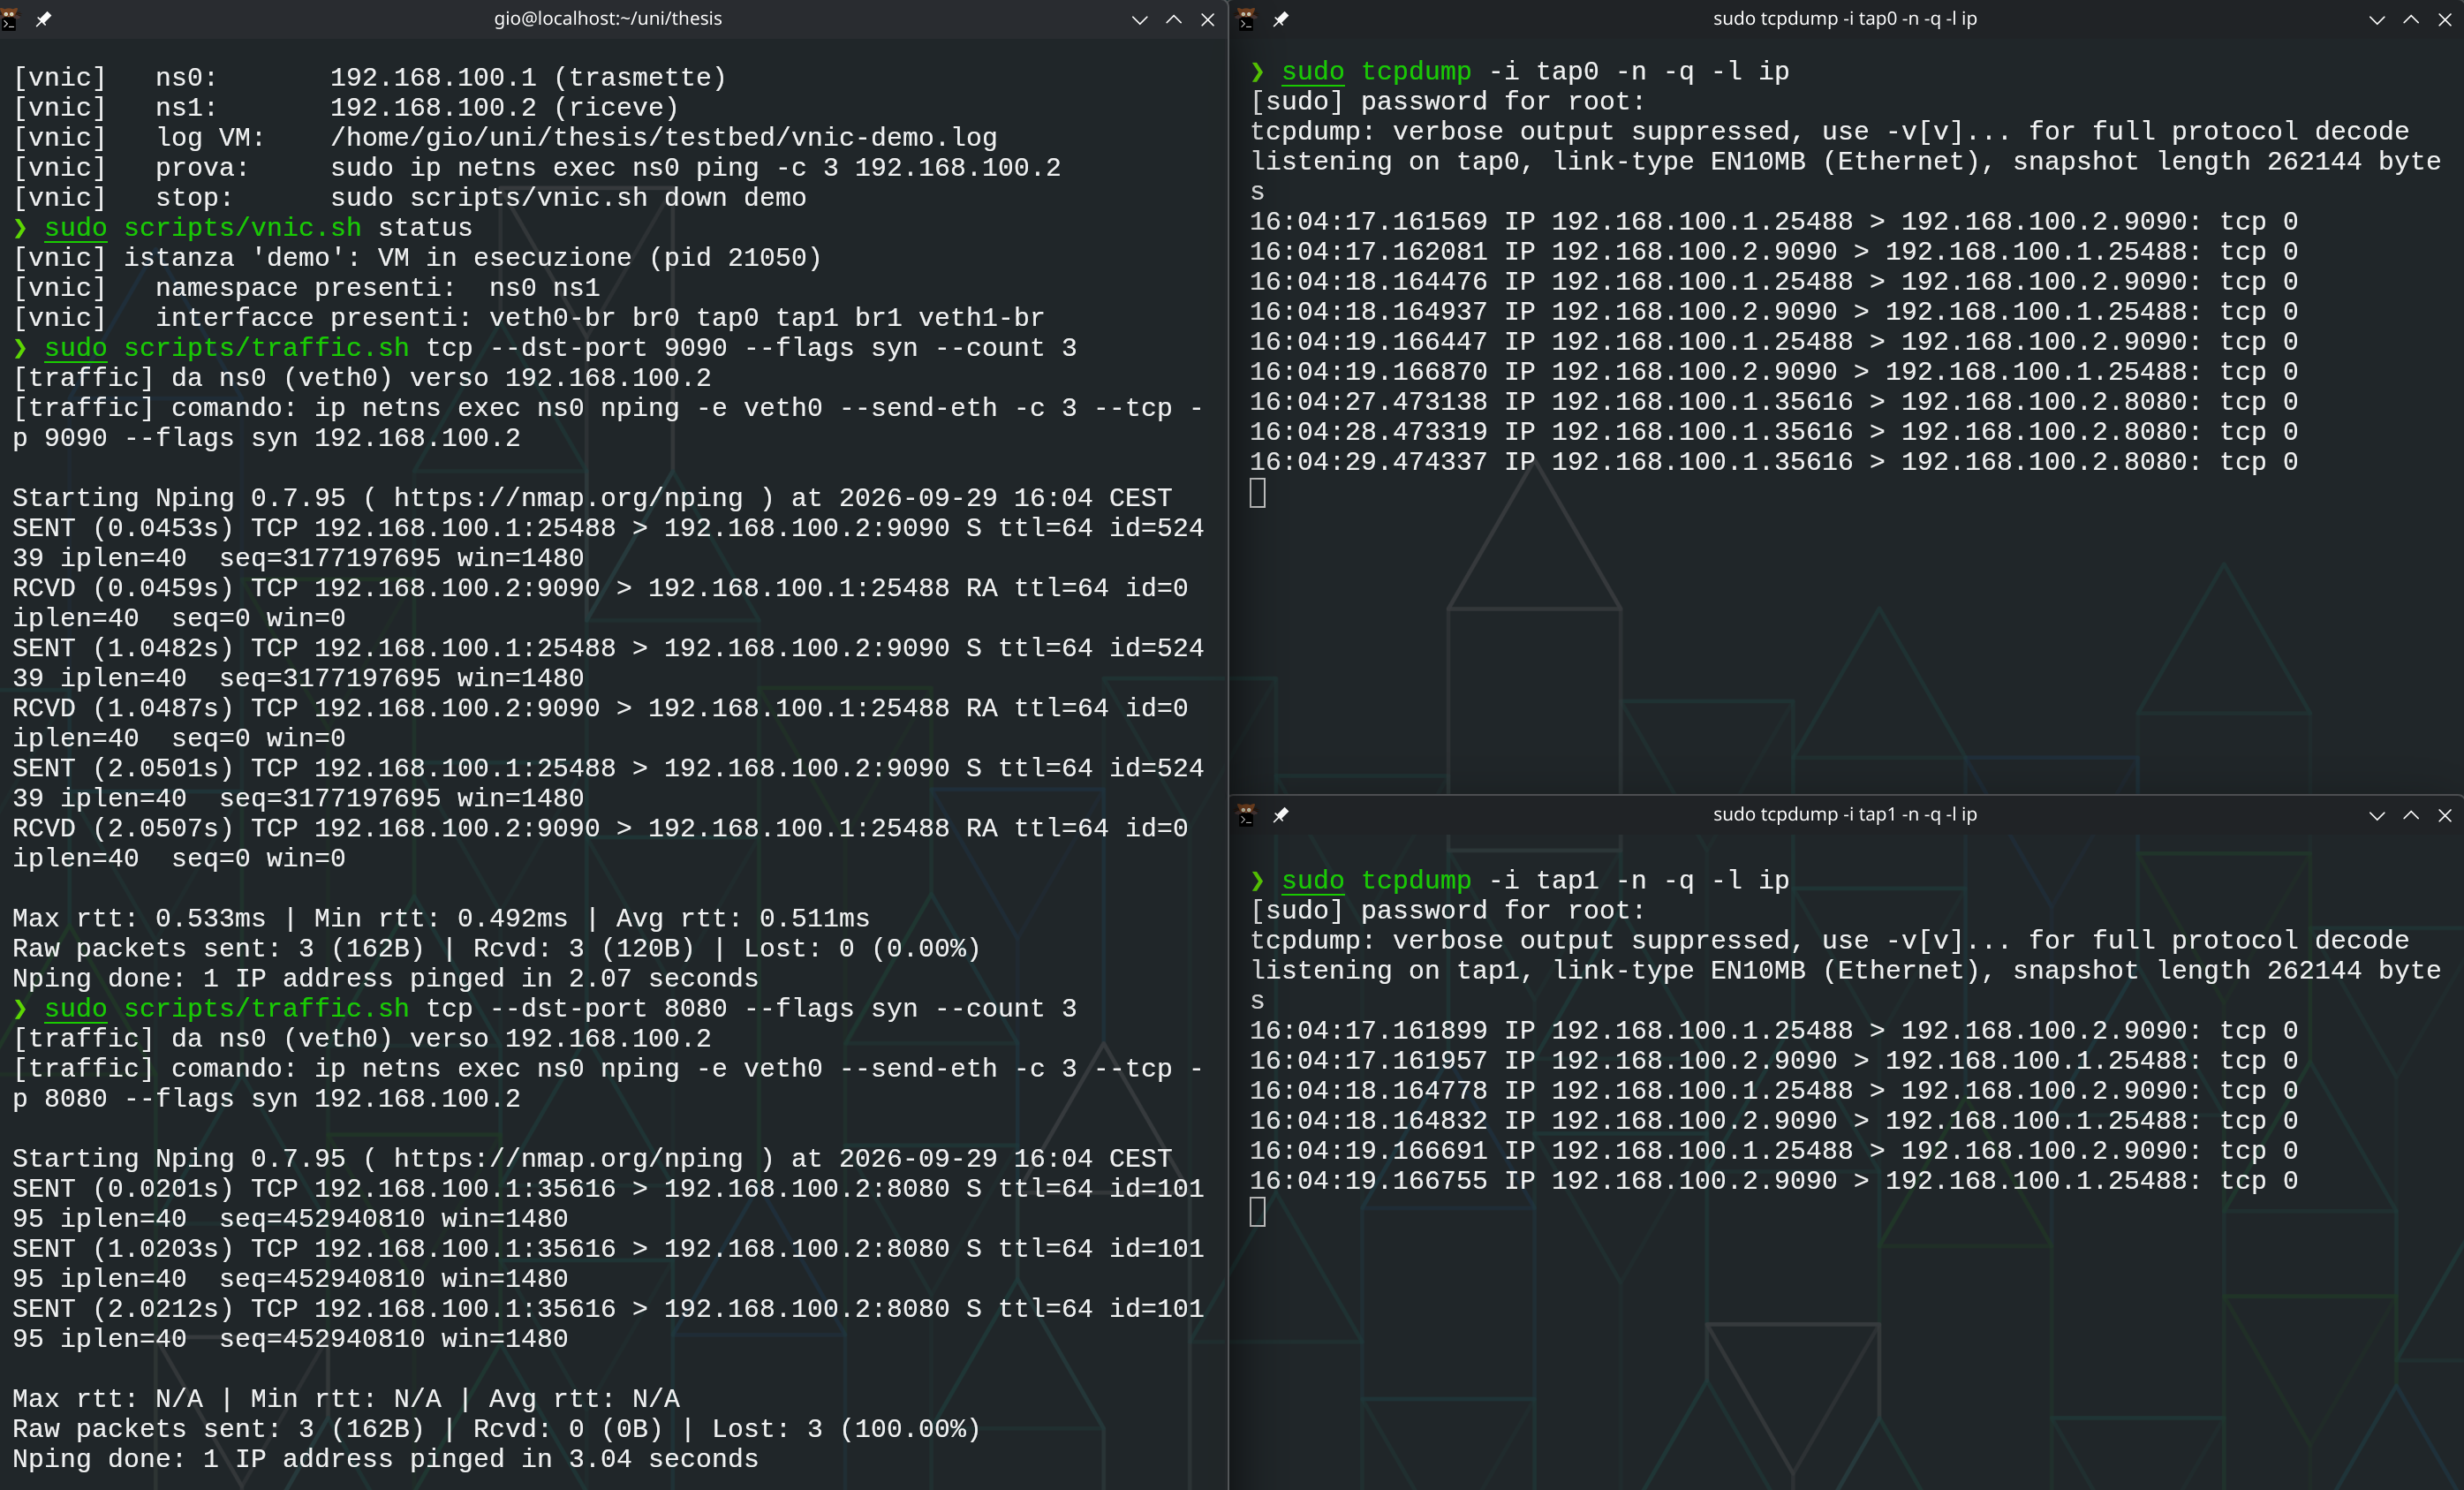
\includegraphics[width=0.9\linewidth]{images/CasoDUso/demo.png}
    \caption{Demo con il filtro in eBPF: a sinistra \texttt{status} e \texttt{traffic.sh}, a destra \texttt{tcpdump} su \texttt{tap0} (in alto) e su \texttt{tap1} (in basso)}
    \label{fig:demo}
\end{figure}

Si può notare che i SYN verso la porta 9090 ricevono il RST mentre quelli verso la porta 8080 restano senza risposta, e infatti \texttt{nping} riporta 3 pacchetti persi su 3. Le catture su \texttt{tap0} e \texttt{tap1} (terminali di destra) mostrano anche dove si fermano. I tre SYN verso la porta 9090 e le relative risposte compaiono su entrambe le TAP, mentre i tre SYN verso la porta 8080 compaiono solo su \texttt{tap0}, quindi sono entrati nella VM ma il programma li ha scartati prima che raggiungessero \texttt{ens4}. Il risultato coincide con le ultime due righe della tabella~\ref{tab:atteso}.

\subsection{Filtro in P4}

Per provare la versione in P4 si ferma l'istanza precedente e se ne avvia una nuova con l'opzione \texttt{-{}-attach-p4} (listing~\ref{lst:p4}). Rispetto all'avvio con il filtro in eBPF, nell'output di \texttt{up} cambiano solo le prime righe, che riguardano la traduzione del programma. In particolare, la prima compare solo se \texttt{p4c-ebpf} non è installato sull'host e vnic usa al suo posto il container. Il traffico verso la porta 8080 viene scartato come con la versione in eBPF.

\noindent\begin{minipage}{\linewidth}
\begin{lstlisting}[style=terminale, caption={Avvio di vnic con il filtro in P4 e traffico verso la porta 8080}, label={lst:p4}]
$ sudo scripts/vnic.sh down demo
[vnic] arresto QEMU (pid: 21050)
[vnic] rimozione infrastruttura host e file temporanei
[vnic] istanza 'demo' rimossa
$ sudo scripts/vnic.sh up demo --attach-p4 examples/tcp-port-filter/tcp_port_filter.p4
[vnic] p4c-ebpf non installato, uso il container p4lang/p4c (al primo avvio scarica l'immagine)
[vnic] traduzione examples/tcp-port-filter/tcp_port_filter.p4 in C (p4c-ebpf) e compilazione
[vnic] infrastruttura lato 0: ns0 (192.168.100.1), veth0, br0, tap0
[...]
[vnic]   programma: examples/tcp-port-filter/tcp_port_filter.p4
[...]
$ sudo scripts/traffic.sh tcp --dst-port 8080 --flags syn --count 3
[...]
Raw packets sent: 3 (162B) | Rcvd: 0 (0B) | Lost: 3 (100.00%)
[...]
$ sudo scripts/vnic.sh down demo
[vnic] arresto QEMU (pid: 22209)
[vnic] rimozione infrastruttura host e file temporanei
[vnic] istanza 'demo' rimossa
\end{lstlisting}
\end{minipage}

\section{Gestione degli errori}\label{sec:errori}

Prima di creare qualsiasi elemento dell'infrastruttura \texttt{up} controlla gli argomenti, i privilegi, le dipendenze, che non ci siano altre istanze attive e infine che il programma esista e si possa compilare. Un input errato viene quindi segnalato subito, senza lasciare niente da rimuovere manualmente. Il listing~\ref{lst:errori} mostra i casi più comuni.

\noindent\begin{minipage}{\linewidth}
\begin{lstlisting}[style=terminale, caption={Risposta di \texttt{vnic.sh} e \texttt{traffic.sh} a input errati}, label={lst:errori}]
$ sudo scripts/vnic.sh up altra
[vnic] errore: un'istanza è già attiva (vnic-demo); usa 'down' prima di un nuovo 'up'
$ sudo scripts/vnic.sh down demo
[...]
$ sudo scripts/vnic.sh up
[vnic] errore: 'up' richiede un nome
Uso: vnic.sh <comando> [opzioni]
[...]
$ sudo scripts/vnic.sh up demo --attach-ebpf a.c --attach-p4 b.p4
[vnic] errore: --attach-ebpf e --attach-p4 sono mutuamente esclusivi
$ sudo scripts/vnic.sh up demo --attach-ebpf nonesiste.c
[vnic] errore: file 'nonesiste.c' non trovato
$ sudo scripts/traffic.sh tcp
[traffic] errore: namespace ns0 assente; avvia prima vnic con 'sudo vnic.sh up <nome>'
\end{lstlisting}
\end{minipage}

Nell'ordine, gli errori riguardano:
\begin{itemize}
    \item \texttt{up} con un'istanza già attiva, non consentito perché i nomi delle interfacce e gli indirizzi sono fissi;
    \item \texttt{up} senza nome. Oltre al messaggio di errore viene stampato l'help completo;
    \item le opzioni \texttt{-{}-attach-ebpf} e \texttt{-{}-attach-p4} usate insieme. Gli argomenti vengono controllati prima dei file, per cui l'errore compare anche se \texttt{a.c} e \texttt{b.p4} non esistono;
    \item caricare un programma inesistente;
    \item \texttt{traffic.sh} senza un'istanza attiva. Lo script si accorge che manca il namespace \texttt{ns0} e indica come avviare vnic.
\end{itemize}

\section{Verifica automatica}\label{sec:verifica}

La demo descritta finora richiede all'utente di interpretare l'output. Per questo ogni esempio in \texttt{examples/} contiene uno script \texttt{verify.sh}, che permette di controllare rapidamente che il tool funzioni sul proprio calcolatore.
\texttt{verify.sh} ripete i test fatti sopra e dà un esito, PASS o FAIL. La versione del programma si sceglie con l'argomento dello script (\texttt{ebpf}, il default, oppure \texttt{p4}). Lo script esegue le seguenti operazioni:
\begin{itemize}
    \item avvia vnic con il programma scelto, usando come nome dell'istanza quello dell'esempio. Subito dopo registra con il comando \texttt{trap} l'esecuzione di \texttt{down} all'uscita, così che l'istanza venga fermata anche se lo script si interrompe per un errore;
    \item avvia due \texttt{tcpdump}, su \texttt{tap0} e su \texttt{tap1}, che per 12 secondi salvano nel file \texttt{.pcap} i pacchetti catturati. Questi file si trovano nella directory temporanea \texttt{/tmp/vnic-verify-<esempio>/};
    \item con \texttt{traffic.sh} invia da \texttt{ns0} sia pacchetti che il programma deve lasciar passare sia pacchetti che deve scartare;
    \item rilegge le catture e conta i pacchetti di ciascun tipo. Quelli che devono passare devono comparire su entrambe le TAP, mentre quelli da scartare solo su \texttt{tap0}.
\end{itemize}

Si tratta del terzo metodo di conteggio descritto nella sezione~\ref{sec:azioni-xdp}. Il listing~\ref{lst:verify-tcp} riporta l'output per l'esempio \texttt{tcp-port-filter}, nella versione in P4.

\noindent\begin{minipage}{\linewidth}
\begin{lstlisting}[style=terminale, caption={Output di \texttt{verify.sh} per l'esempio \texttt{tcp-port-filter}, versione in P4}, label={lst:verify-tcp}]
$ sudo examples/tcp-port-filter/verify.sh p4
[verify] avvio vnic con examples/tcp-port-filter/tcp_port_filter.p4
[vnic] p4c-ebpf non installato, uso il container p4lang/p4c (al primo avvio scarica l'immagine)
[vnic] traduzione examples/tcp-port-filter/tcp_port_filter.p4 in C (p4c-ebpf) e compilazione
[vnic] infrastruttura lato 0: ns0 (192.168.100.1), veth0, br0, tap0
[vnic] infrastruttura lato 1: ns1 (192.168.100.2), veth1, br1, tap1
[vnic] preparazione VM: cloud-init, seed.iso, overlay dell'immagine base
[vnic] avvio VM, attesa boot e cloud-init (30s circa)...
[vnic] VM pronta (completato in 33s)
[vnic] istanza 'tcp-port-filter' pronta
[vnic]   programma: examples/tcp-port-filter/tcp_port_filter.p4
[vnic]   ns0:       192.168.100.1 (trasmette)
[vnic]   ns1:       192.168.100.2 (riceve)
[vnic]   log VM:    /home/gio/uni/thesis/testbed/vnic-tcp-port-filter.log
[vnic]   prova:     sudo ip netns exec ns0 ping -c 3 192.168.100.2
[vnic]   stop:      sudo scripts/vnic.sh down tcp-port-filter
[verify] cattura su tap0 e tap1 per 12s
[verify] TCP: 3 SYN ns0 -> ns1:9090 (devono passare)
[verify] TCP: 3 SYN ns0 -> ns1:8080 (devono essere scartati)
[verify] porta 9090: tap0=3 tap1=3 | porta 8080: tap0=3 tap1=0
[verify] PASS: porta 9090 raggiungibile, porta 8080 bloccata
[vnic] arresto QEMU (pid: 23441)
[vnic] rimozione infrastruttura host e file temporanei
[vnic] istanza 'tcp-port-filter' rimossa
\end{lstlisting}
\end{minipage}

Oltre all'output stampato da vnic per i comandi \texttt{up} e \texttt{down} è presente quello di \texttt{verify.sh}, che descrive il traffico inviato e il risultato del conteggio. Lo script conta solo i pacchetti diretti alle due porte, cioè i SYN e non le risposte. Si può notare che i 3 SYN verso la porta 9090 compaiono su entrambe le TAP, mentre i 3 verso la porta 8080 solo su \texttt{tap0}, come nella demo manuale.

L'altro esempio, \texttt{drop-udp}, scarta tutti i pacchetti UDP su IPv4 e lascia passare il resto. È lo stesso filtro usato nel test manuale (\texttt{docs/VM-test.md}, sezione~\ref{sec:processo}). Il suo \texttt{verify.sh} invia da \texttt{ns0} a \texttt{ns1} 5 ping e un pacchetto UDP diretto alla porta 9999, e conta i pacchetti ICMP e UDP catturati sulle due TAP. Il listing~\ref{lst:verify-udp} ne riporta l'output con la versione in eBPF senza le righe stampate da vnic.

\noindent\begin{minipage}{\linewidth}
\begin{lstlisting}[style=terminale, caption={Output di \texttt{verify.sh} per l'esempio \texttt{drop-udp}, versione in eBPF}, label={lst:verify-udp}]
$ sudo examples/drop-udp/verify.sh
[verify] avvio vnic con examples/drop-udp/drop_udp.c
[...]
[verify] cattura su tap0 e tap1 per 12s
[verify] ICMP: 5 echo request ns0 -> ns1 (devono passare)
[verify] UDP: 1 pacchetto ns0 -> ns1:9999 (deve essere scartato)
[verify] ICMP: tap0=10 tap1=10 | UDP: tap0=1 tap1=0
[verify] PASS: ICMP attraversa la VM, UDP viene scartato
[...]
\end{lstlisting}
\end{minipage}

I pacchetti ICMP registrati sono 10 su entrambe le TAP, 5 richieste e 5 risposte, mentre il pacchetto UDP compare solo su \texttt{tap0}, quindi è entrato nella VM ed è stato scartato dal programma, come atteso.

Al termine le catture restano in \texttt{/tmp/vnic-verify-<esempio>/}, dove in caso di esito negativo si possono analizzare con \texttt{tcpdump -r <file>}. Oltre a verificare il funzionamento di vnic, gli esempi servono anche come punto di partenza per nuovi programmi, copiando una delle cartelle e modificando la logica del filtro e il traffico inviato da \texttt{verify.sh}.
